\documentclass{article}
\usepackage[utf8]{inputenc}
\usepackage{tikz}
\usetikzlibrary{shapes.geometric, arrows}
\tikzstyle{block} = [rectangle, rounded corners, minimum width=3cm, minimum height=1cm,text centered, draw=black]
\tikzstyle{arrow} = [thick,->,>=stealth]


\title{CS 1530 - HW 1}
\author{Gerard McGlone }
\date{February 5 2019}



\begin{document}

\maketitle

\section{}
1. What is the SDLC and define its various stages?\newline

\noindent The SDLC stands for "Software Development Life Cycle", which is a generalized procedure for producing and maintaining software.  This procedure is commonly broken into the following steps:
\begin{enumerate}
    \item Requirements Analysis
    \item Design
    \item Implementation (Engineering)
    \item Testing
    \item Maintain/Evolve
\end{enumerate}
The steps above can be completed in linear-sequential fashion, iteratively repeating certain steps, or in a hybridized form.  Different flavors of the SDLC appeal in different situations, with no single solution being the best for all software projects.\newline

Requirements Analysis, often the first thing carried out, is the gathering of functional and non-functional requirements of the proposed software.  Requirements are typically written in English, and detail what exactly the software needs to do (its functional reqs) and how exactly it needs to be (its non-functional reqs).  The Design stage consists of the determining what the solution is going to look like.  Here, we often want to map out the logical structure of the solution to the problem and figure out what our technology stack will consist of.  Through extensive UML diagramming, we can make the implementation stage easier and more straightforward.  In the implementation stage, we code the solution.  Here we implement interfaces and fill in class definitions as were specified in the previous (design) stage.  This stage is often the easy stage if the other stages are carried out well.  In the testing stage, we verify that we are building the software right.  We test for quality, performance, usability before releasing the software.  In the final stage of the SDLC, we maintain the software.  This consists of providing support to software through updates, new versions of it, etc.  This stage often consists of major changes and transformations of the software as well.

\section{}
\subsection{Three varieties of the SDLC}
1. \textit{Waterfall} \\ \\
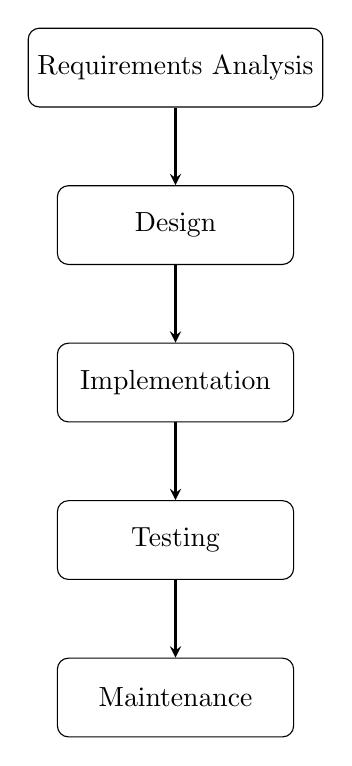
\begin{tikzpicture}[node distance=2cm]
\node (reqs) [block] {Requirements Analysis};
\node (des) [block, below of=reqs] {Design};
\node (imp) [block, below of=des] {Implementation};
\node (tst) [block, below of=imp] {Testing};
\node (mntn) [block, below of=tst] {Maintenance};

\draw [arrow] (reqs) -- (des);
\draw [arrow] (des) -- (imp);
\draw [arrow] (imp) -- (tst);
\draw [arrow] (tst) -- (mntn);
\end{tikzpicture} \\ \\
This model is a linear-sequential implementation of the aforementioned steps in SDLC.  Each step is carried to completion before advancing to the next step. \\

2. \textit{Spiral}\\ \\
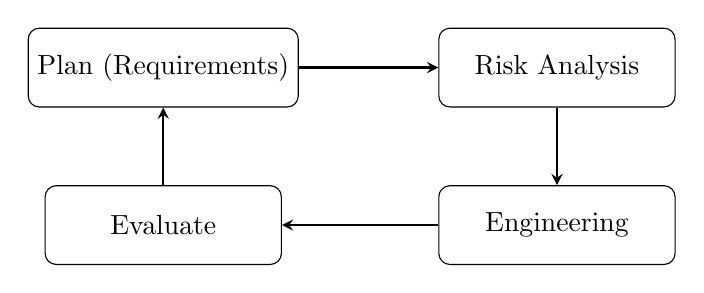
\begin{tikzpicture}[node distance=2cm]
\node (reqs) [block] {Plan (Requirements)};
\node (rska) [block, right of=reqs, xshift=3cm] {Risk Analysis};
\node (eval) [block, below of=reqs] {Evaluate};
\node (imp) [block, right of=eval, xshift=3cm] {Engineering};

\draw [arrow] (reqs) -- (rska);
\draw [arrow] (rska) -- (imp);
\draw [arrow] (imp) -- (eval);
\draw [arrow] (eval) -- (reqs);
\end{tikzpicture} \\ \\
The spiral model typically begins in some sort of planning stage where requirements are gathered, and then advances sequentially to risk analysis where prototyping and risk reduction is done, and then to engineering where the coding/unit testing is done, and then finally to an evaluation stage where the overall progress is considered and scrutinized. \\

3. \textit{Iterative} \\ \\
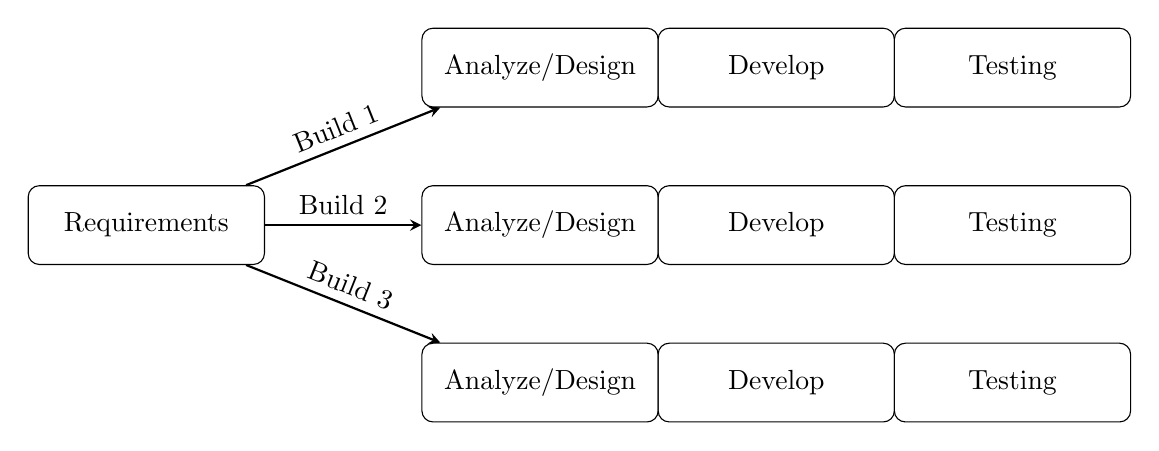
\begin{tikzpicture} [node distance=2cm]
\node (reqs) [block, yshift=-2cm] {Requirements};
\node (des1) [block, right of=reqs, yshift=2cm, xshift=3cm ] {Analyze/Design};
\node (des2) [block, right of=reqs, xshift=3cm] {Analyze/Design};
\node (des3) [block, right of=reqs, xshift=3cm, yshift=-2cm] {Analyze/Design};
\node (dev1) [block, right of=des1, xshift=1cm] {Develop};
\node (dev2) [block, right of=des2, xshift=1cm] {Develop};
\node (dev3) [block, right of=des3, xshift=1cm] {Develop};
\node (tst1) [block, right of=dev1, xshift=1cm] {Testing};
\node (tst2) [block, right of=dev2, xshift=1cm] {Testing};
\node (tst3) [block, right of=dev3, xshift=1cm] {Testing};

\draw [arrow] (reqs) -- (des1) node[midway, sloped, above] {Build 1};
\draw [arrow] (reqs) --  (des2) node[midway, sloped, above] {Build 2};
\draw [arrow] (reqs) --  (des3) node[midway, sloped, above] {Build 3};
\end{tikzpicture} \\ \\
The iterative model typically begins with requirements, but they do not need to be fully specified like in other models.  In this model we typically implement the overall solution piece by piece, reviewing and improving upon it at each stage.  The requirements may be changed in between build prototypes, but at each stage we are designing, developing, and testing.

\subsection{Advantages and Disadvantages}
The waterfall model is advantageous when we have full specification of the requirements and a good design plan, because then the implementation and testing stage will be easy.  If we have a very good idea of what we need without too much risk, waterfall model is good.  Moreover, if the project is short, then the waterfall model is typically good because we probably understand the whole project in terms of requirements. The spiral model is advantageous when we need to conduct a lot of risk analysis.  It is flexible like the Iterative model, but there is a higher emphasis on risk analysis and risk reduction.  For a long project with ambiguous requirements, the spiral model is a good choice.  The iterative model is advantageous when a team is using new technology, because as they are learning the tech better, they can better improve upon builds of the prototype.

One of the disadvantages of the waterfall model is that it doesn't support dynamic plans.  If some aspects of our requirements are uncertain or have a lot of risk, the waterfall model isn't best supported to handle these.  One of the disadvantages of the Iterative model is that it might be inefficient if the project is short and we know our technology well.  We might not need to build the extra prototypes.  Similarly, if we understand our project well and it's going to be short, the spiral model might also be inefficient and costly.
\section{}
\subsection{What is Agile?}
Agile methodology combines aspects of iterative methodology with its own new ideas.  Agile builds the software in short 1-4 week increments, where a workable part of the product can be delivered every 1-4 weeks.  Rather than develop all at once, Agile develops and tests in increments to meet changing business needs; it is indeed a flexible and dynamic option.

\subsection{3 main flavors of Agile}
\begin{enumerate}
    \item SCRUM - cycles broken down by time
    \item Kanban - cycles broken down by number of tasks per job
    \item XP - Extreme programming to ensure it is of the highest quality. TDD and pair programming are examples.
\end{enumerate}

\subsection{Definitions of Various Sprint Meetings}
\begin{itemize}
    \item Sprint Planning - In this meeting, we allot 1-4 weeks to complete a various assortment of individual tasks, all of which together contribute to some greater part of the system.  We assign points to each task with the more involved/complex tasks getting more points.
    \item Daily Standup - This meeting takes place everyday and ensures that progress is being made on the individual tasks of a given sprint.  If meetings are had everyday, that will ensure that no one person gets stuck for days on something with nobody knowing about it.  Getting stuck for days without help is expensive to the organization, and daily standups minimize this.  They also help to make sure we are being timely with the progress of our sprint.
    \item Sprint Review - This meeting is conducted when we finish a sprint, whereby we ensure the completion and quality of each of the tasks in our sprint.  Each person talks about how they're done what they've been assigned.  
    \item Sprint Retrospective - This meeting is the last meeting of a sprint and is for figuring out what could be improved upon.  We often do things that could be done better, so in this meeting we discuss how we can save time and energy on our sprints, so we can be more efficient.
    
    \subsection{What are the various SCRUM teams and their roles?}
    \begin{itemize}
        \item Product Owner - this member owns the product and is the most financially invested in the project.  As such, they typically care about the timeliness, efficiency, completion, and other aspects of the project.  They oversee that the project is going well, and have direct interests in the end results of it.  They will probably be reviewing what is delivered in each sprint (or every few sprints).  
        \item SCRUM Master - This member is responsible for making sure each individual sprint is carried out efficiently and to completion.  They stay on top of the individual team members to make sure their work is being done as it should, and they also report the progress and respond to the Product Owner
        \item SCRUM team member - A team member is one who undertakes completing or assuring the quality of features.  This could be someone helping with requirements and documentation, a programmer implementing a solution, testers looking to assure quality. 
    \end{itemize}
\end{itemize}
\subsection{What are product and sprint backlogs?}
The product backlog is a list of features/tasks that need to be completed as apart of the project.  With each sprint, we move a specific selection of tasks in the product backlog into the sprint backlog.  The features of a sprint are defined precisely by the sprint backlog in its initial state.  Once we complete all the features in the sprint backlog, we complete the sprint.
\section{}
\subsection{Functional and Non-Functional Requirements}
Functional requirements describe what the software needs to do.  In any given piece of software, there will be some sort of output based on input (including null input), which is its essential 'function'. We want to document all of its required, functional behaviors into a compiled list, known as its functional requirements.  Non-Functional requirements describe how software needs to be.  It details what in addition to its essential function we will need.  In almost any given piece of software, there will be some sort of user, so how the user interacts with it and ensuring a quality user experience will be important.  

\subsection{Examples}
Imagine a piece of software that takes a picture of your face and determines whether or not you are ugly.  Below are five functional and five non-functional requirements, respectively.  
\begin{enumerate}
    \item Has a homepage
    \item Takes Picture of Face
    \item Shows user the Picture of the face that it took.
    \item Determines whether or not the user is ugly
    \item Saves the results in an exportable format
\end{enumerate} 
--------------------------------------------------------------------------------
\begin{enumerate}
    \item Friendly and navigable homepage
    \item Image capturing is secure.  That is, when a user takes a picture only they view/access it.
    \item Platform is scaleable.  Many, many people can use this at any given time.
    \item Platform is fast.  Ugliness results are generated fast so that user isn't waiting.
    \item Exporting data is ensured to be easy with a friendly and simple interface.
\end{enumerate}


\end{document}

